\subsection{The TorPath Protocol}

The TorPath protocol assigns Tor circuits to clients, replacing the usual Tor
directory servers with \textit{assignment servers}, which form decentralized
\textit{consensus groups}. The protocol guarantees that no participant on a 
circuit can identify all other participants, and that each circuit includes a 
publicly verifiable signature. We use TorPath to ``sign'' each TorCoin, so that 
anyone can verify a TorCoin's validity by comparing its signature to a global
history of consensus groups.

\subsubsection{Requirements:}
The TorPath protocol adheres to the following constraints:

\begin{itemize}   
\item No client can generate its own circuit.
\item Every circuit has a unique, publicly-verifiable signature.
\item No client can know the circuit of another client.
\end{itemize}

\subsubsection{Protocol Outline:}

The TorPath protocol consists of three sequential steps:

\begin{enumerate}
\item \textbf{Group Initialization.} Assignment servers form a \textit{consensus 
group}. Clients and available relays provide public keys to join the group.

\item \textbf{Verifiable Shuffle.} The consensus group performs a decentralized, 
verifiable shuffle of all the public keys, resulting in a circuit assignment for
each client.

\item \textbf{Path Lookup.} The assignment servers publish the result of the 
shuffle, such that each client can identify only its entry relay, and each 
relay can identify only its immediate neighbor(s) in the circuit.
\end{enumerate}

\paragraph{Stage 1 -- Group Initialization:}

A consensus group is formed when a suitable quorum of assignment servers come
together to assign circuits to recently registered clients.
For example, if there are 10 assignment servers in the network,
we might require at least 6 of them to participate
in forming each consensus group.
The assignment servers can modulate the size -- and hence anonymity --
represented by each consensus group,
by waiting until there are some configurable number $n$ of clients
registered before proceeding to the next stage.
Different categories of consensus groups might use different values of $n$,
allowing clients to trade anonymity for wait time.
Groups with larger values of $n$ would provide a larger
anonymity set, at the expense of longer circuit setup times.

\begin{figure}[htbp]
  \centering
  \subfloat[]{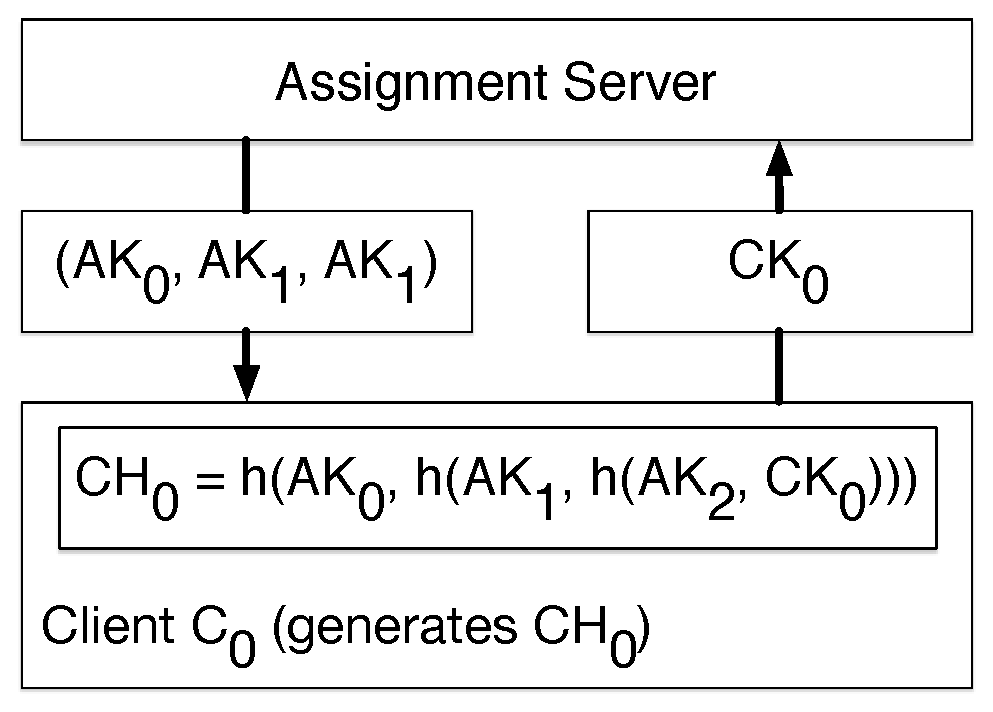
\includegraphics[width=.49\textwidth]{group_formation_2.pdf}}
  \subfloat[]{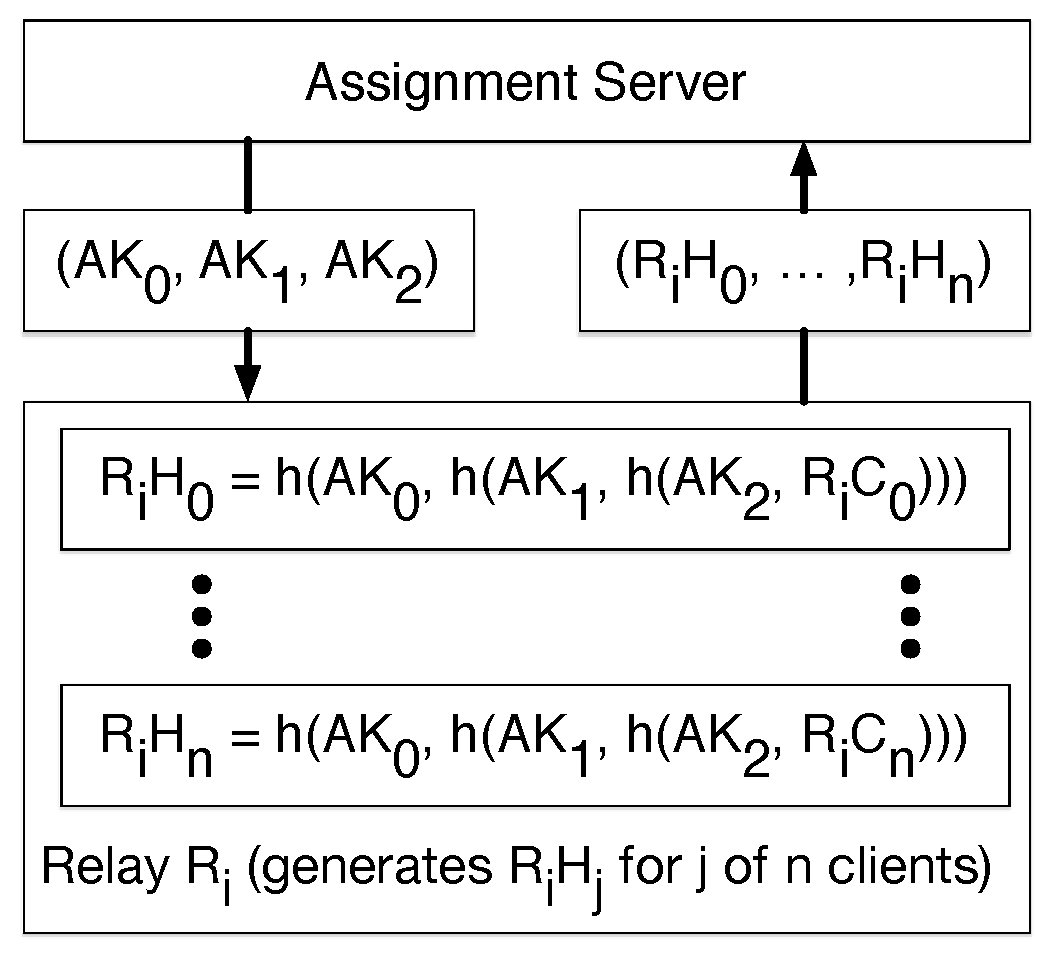
\includegraphics[width=.49\textwidth]{group_formation_3.pdf}}
  
  \caption{Both relays and clients use onion-encryption to encrypt their own   temporary public keys with the public keys of all the assignment servers in the group. (a) Client generates one keypair. The public key is sent onion-encrypted to the server. (b) Each relay generates multiple keypairs (for different clients and positions) as instructed by the assignment servers.}
  
  \label{figure:transfer}
\end{figure}

A consensus group forms in three steps:

\begin{enumerate} 

\item \textbf{Each assignment server} shares its public key with its group
members, and broadcasts these public keys to all clients and relays
connected to it.

\item \textbf{Each client} connects to one assignment server in the group. The
client then generates a temporary private and public key pair.
The client onion-encrypts its temporary public key
with the public keys of all assignment
servers in the group, resulting in a ciphertext that each server can only partially
decrypt. The client submits this ciphertext to its assignment server.

\item \textbf{Each relay} can act as an entry, middle, and/or exit relay, and
it chooses which position(s) to service. The number of available
relays available for a given position (especially exit relays)
may often be less than the number of clients in the group needing circuits.
To ensure parity between
clients and relays for each position, each assignment server instructs its relays to generate a
sufficient number of temporary keys for each position. The relay server uses
onion-encryption to generate $n$ ciphertexts from $n$ temporary public keys.
The relay packages these ciphertexts by position
and sends them to its upstream assignment server.
\end{enumerate}

Figure \ref{figure:transfer} illustrates Steps 2 and 3.

We can represent the temporary keys as an $n \times 4$ matrix $M$ for $n$
clients, where each row corresponds to a client and its three relays (see
Figure \ref{figure:shuffle}).

\begin{figure}[t]
  \centering
    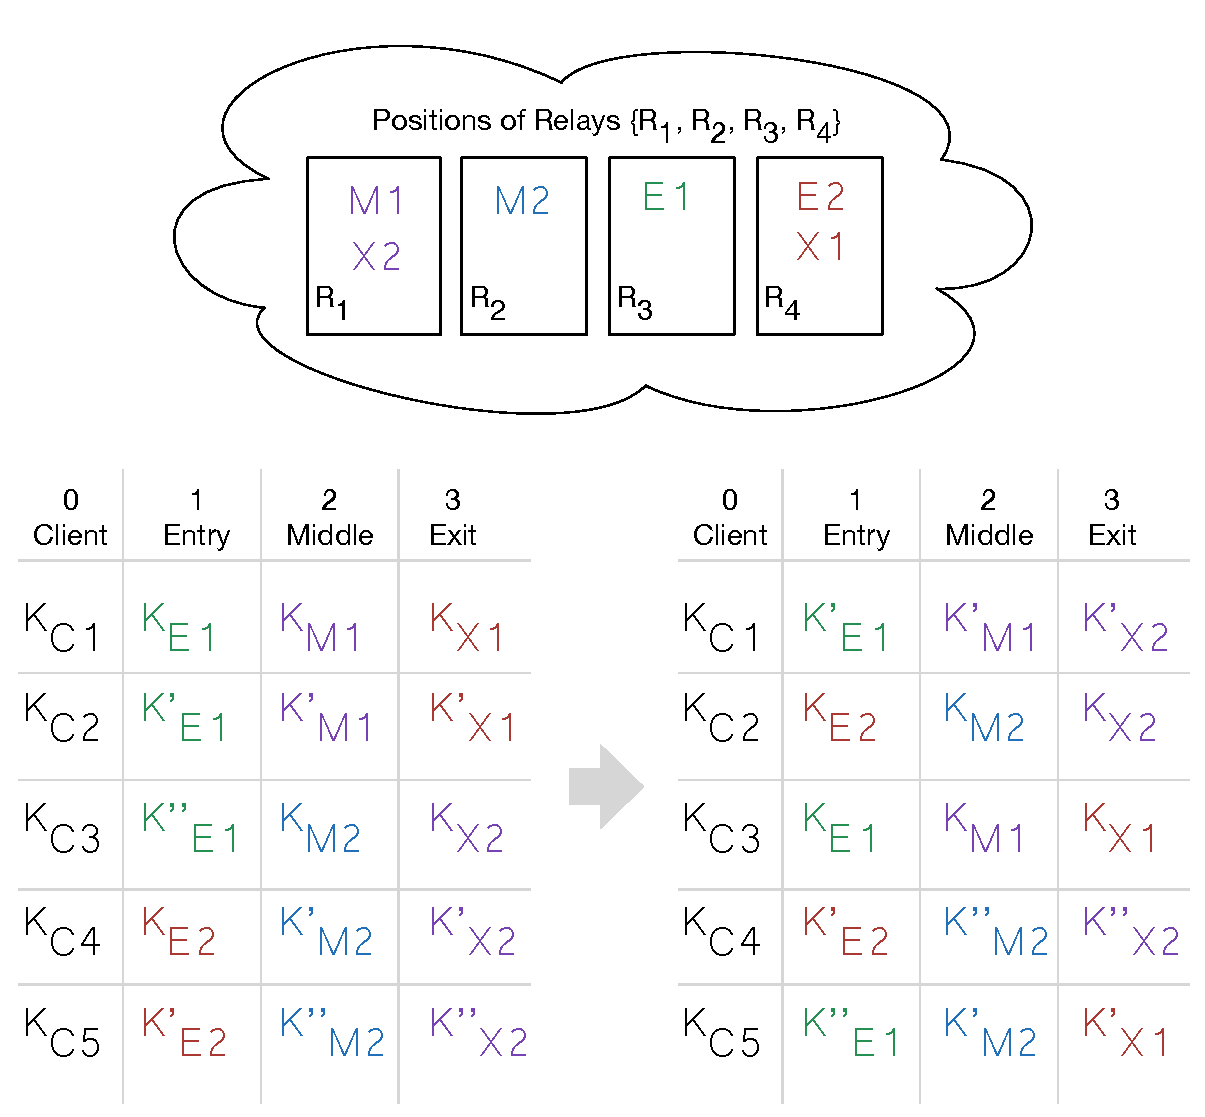
\includegraphics[scale=.6]{shuffle_total.pdf}
  \caption{
    Example matrix shuffle with 5 clients ($C_1$, $C_2$, $C_3$, $C_4$ and $C_5$) 
    and 4 relays (purple, blue, green, red). Each relay $R_i$ generates a number 
    of public keys $K_p^i$ for each circuit position $p \in {E, M, X}$, as 
    instructed by its assignment server. Here, each client $C_j$ is assigned the 
    circuit represented by the $j^{th}$ row of the shuffled matrix. 
  }
  \label{figure:shuffle}
\end{figure}



\paragraph{Stage 2 -- Verifiable Shuffle:}
The consensus group now shuffles
each column of the temporary key matrix independently,
using a verifiable shuffling algorithm
such as the Neff Shuffle~\cite{neff2001verifiable}),
and jointly decrypts the shuffled keys.
Each row in the public result matrix now contains
a random 4-tuple of temporary public keys representing one circuit:
namely the client and the three relays serving that client.
The assignment servers collectively sign and publish the resulting matrix to a
public log, accessible by all clients and relays.
Although everyone learns which four temporary public keys
represent the participants of each circuit,
the verifiable shuffle prevents anyone except a given key's owner from learning
{\em which} participating client or relay owns each of these temporary keys.

\paragraph{Stage 3 -- Path Lookup:}
In the final step of the algorithm, each client obtains the
IP address of its entry relay, and each relay obtains the IP address of its
neighbor(s) on the circuit. The path lookup algorithm ensures that each client
and relay can obtain {\em only} the IP addresses
of its neighbors in the circuit.

Each client encrypts its own IP using the public key of its neighbor.
The client
forms a tuple (public key, encrypted IP) as shown in table
\ref{table:message_format}.
The client onion-encrypts this tuple and sends it to the
assignment servers.
Each relay follows the same procedure, for every key in the
matrix belonging to it.

The assignment servers shuffle this new list of tuples. Each
client and relay now finds its neighbors in the matrix by locating the tuples
containing the public keys it needs. Finally,
each participant decrypts the relevant cells using
its private key, revealing the IP address of its circuit neighbor(s).

Now all clients in the consensus group have a usable Tor circuit.

{\renewcommand{\arraystretch}{2}
\begin{table}[h]
\centering
  \begin{tabular}{ |c | c| }
  \hline
  \textbf{Sender} & \textbf{Message Tuple} \\ \hline
  Client & ($K^{i}_{C}$, $\{IP^{i}_{C}\}_{K^{i}_{E}}$) \\ \hline
  Entry relay & ($K^{i}_{E}$, $\{IP^{i}_{E}\}_{K^{i}_{C}}$, $\{IP^{i}_{E}\}_{K^{i}_{M}}$) \\ \hline
  Middle relay & ($K^{i}_{M}$, $\{IP^{i}_{M}\}_{K^{i}_{E}}$, $\{IP^{i}_{M}\}_{K^{i}_{X}}$) \\ \hline
  Exit relay & ($K^{i}_{X}$, $\{IP^{i}_{X}\}_{K^{i}_{M}}$) \\ \hline
  \end{tabular}
  \vspace{.5cm}

  \caption{Each participant in a circuit sends its message 
  tuple onion-encrypted to the server. $\{X\}_{Y}$ denotes X encrypted with Y.}
  \label{table:message_format}
\end{table}

\vspace{-1cm}

Each circuit formed by a consensus group obtains a unique Circuit Identifier,
which is an ordered pair consisting of the hash of the matrix $M$ and the
row number $i$ of the circuit within $M$: $CS_i = (\mathrm{Hash}(M), i)$. This
identifier will be used in the TorCoin algorithm,
together with signatures using the four anonymous temporary public keys
comprising that row of $M$,
to prove that TorCoins were
minted by circuits assigned in consensus groups.

\subsection{TorPath Security Considerations} 

\paragraph{Anonymity:} The TorPath protocol guarantees that no single
relay knows any client's entire circuit. If malicious
clients or relays collude, they may be able to shrink the anonymity set to
the set of honest relays and clients in the consensus group. 
Groups can have varying sizes, however,
allowing clients to choose a desired balance
between anonymity threshold and circuit assignment delay.

\paragraph{Group Formation:}
The TorPath protocol's random circuit selection mechanism prevents
colluding clients and relays from deterministically placing themselves
in the same circuit,
provided not too many participants in each group collude.
Even if half of the temporary keys in matrix $M$
are held by colluding participants, for example,
only $1/2^4 = 1/16$ of the assigned circuits
will be compromised and able to mint (a limited number of)
TorCoins without performing useful work.
We could add further protection
against ``flash mobs'' of colluding participants
by randomizing group assignment across longer time periods,
instead of using temporal locality as the only grouping criterion.

\paragraph{Circuit Diversity:}  
TorCoin's Neff shuffle could assign the same relay to one circuit in multiple
positions: e.g., choose the same physical relay as both entry and middle
relays. With a reasonable number of participating relays, however,
it should be extremely unlikely that one relay gets assigned
to {\em all three} positions on the same circuit.
In any case, the risk of accidental relay duplication on one path
should not be substantially greater than the risk
Tor users already face of randomly placing multiple relays
owned by the {\em same operator} on a circuit.
We anticipate that privacy-preserving {\em independence testing} techniques
could be adapted to detect and reject circuits in which the same relay
(or operator) appears multiple times~\cite{zhai13untold},
but we leave this challenge to future work.
